% intro 
The simulations of blood flows in a nozzle, pump, and IVC with FEM and PFEM-2 are conducted and compared with experimental results \cite{fda_res,fda_nozzle ,fda_pump,gallagher_exp}. The fluid is assumed to be blood analog Newtonian fluid. For the nozzle and pump flows, the fluid density and viscosity are set to be $\rho= 1035$ kg/m\textsuperscript{3} and $\mu =3.5\times10^{-3}$ N-s/m\textsuperscript{2}, where as for the IVC flows, the density and viscosity are $\rho=1817$ kg/m\textsuperscript{3}, $\mu=5.83\times10^{-3}$ N-s/m\textsuperscript{2} for resting condition and $\mu=5.49\times10^{-3}$ N-s/m\textsuperscript{2} for exercising condition. 

\subsection{Blood Nozzle}

%  nozzle intro
The 3D simplified nozzle proposed by FDA consists of four parts containing characteristics of some blood-conveying medical devices. There are inlet and outlet tubes with diameter $0.012$ m, as well as a cone-shaped converging tube connecting the inlet tube with the nozzle throat with diameter $0.004$ m as shown in Fig.~\ref{fig:nozzlegeo1}. The flow experiences a gradual contraction of area from the inlet tube to the throat, then a sudden expansion of area right after the throat to the outlet tube (see Fig.~\ref{fig:nozzlegeo2}). The z coordinate along the axial direction has origin at the exit of the nozzle throat. The flow at Reynolds number $3500$ with flowrate $3.64\times10^{-5}$ m\textsuperscript{3}/s corresponding to turbulent flow regime is analyzed, where the Reynolds number is defined with the flow rate and the diameter at the throat. 

%*** ADD COMPUTATIONAL DOMAIN TO SHOW THAT IT IS A 3D MODEL ***
% keywords like '3D simplified nozzle', '3D domain', 'tetrahedral element' should be sufficient indications that this is a 3D model

\begin{figure}[htbp]
    \centering
    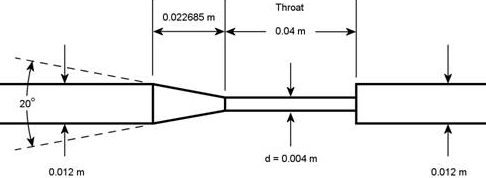
\includegraphics[width=3.3in]{imgs/nozzle_pump/nozzle_geo_2.png}
    \caption{The dimension of the idealized nozzle model proposed by FDA.}
    \label{fig:nozzlegeo1}
\end{figure}
\begin{figure}[htbp]
    \centering
    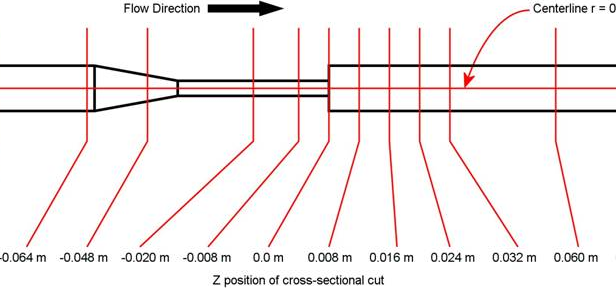
\includegraphics[width=3.3in]{imgs/nozzle_pump/nozzle_CS_2.png}
    \caption{The flow direction and the definition of the axial coordinate z.}
    \label{fig:nozzlegeo2}
\end{figure}


%  nozzle simulation setup
For the set up of the numerical simulation a 3D domain is defined from $z=-0.18$ m to $z=0.18$ m. The prescribed uniformly distributed velocity profile is imposed at the inlet while the pressure is constant at outlet. The Large Eddy Simulation (LES) Smagorinsky model is chosen to deal with the turbulence regime in the nozzle, and the Smagorinsky coefficient is set to be $0.1$ (empirically derived for flows in pipes). The turbulence intensity at the inlet is set to be $5$\% (see Smirnov's turbulence synthesis method~\cite{Smirnov2001}). There are two different kinds of meshes considered in this study: mesh A with a more uniform mesh size in the outlet tube, and mesh B has mesh refinement at certain area (see Fig.~\ref{fig:nozzlemesh}). The mesh A has minimum mesh size $0.2$ mm and a total of $8.61$ million tetrahedral elements. The mesh B has mostly coarser elements in the outlet tube than mesh A, but with mesh refinement near the exit of the throat. The minimum mesh size of mesh B is $0.1$ mm with total of $1.13$ million tetrahedral elements. By using two distinct meshes the sensitivity of the FEM and PFEM-2 methods to the mesh resolution may be observed. Simulations with different CFL number will also be done to examine the influence of the time step size with these two methods.

\begin{figure}[htbp]
    \centering
    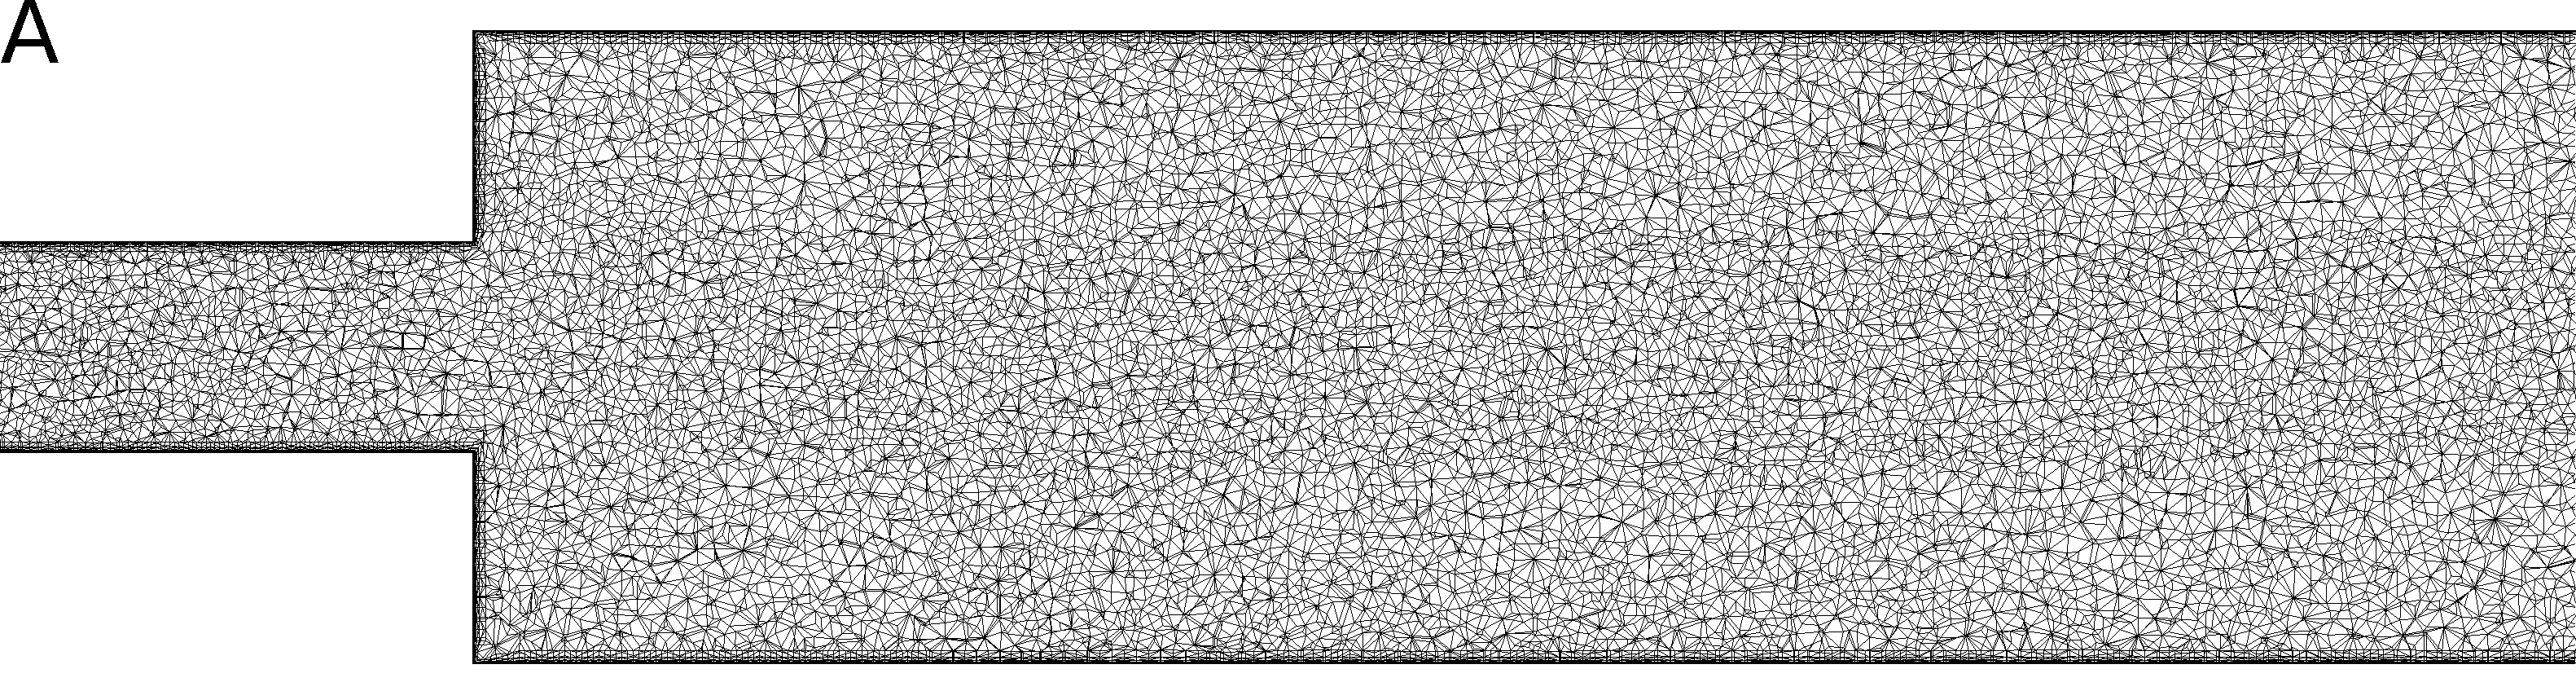
\includegraphics[width=3.2in]{imgs/nozzle_pump/nozzle_fmesh_2.pdf}
    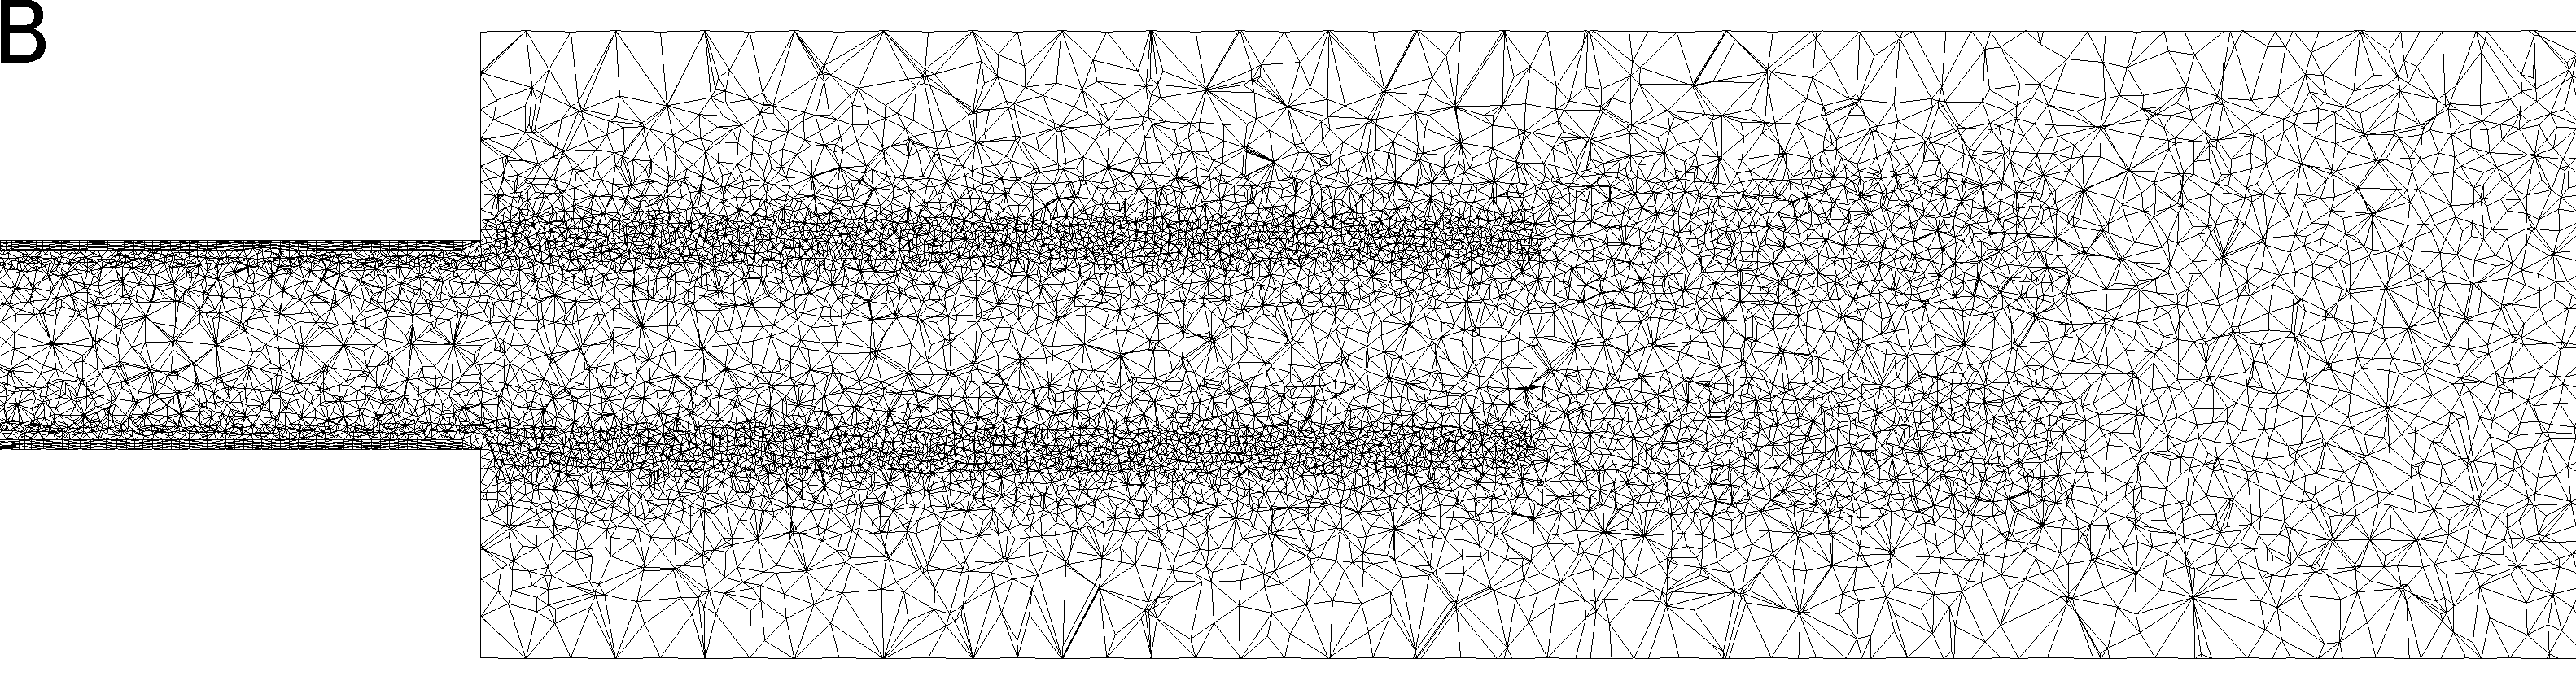
\includegraphics[width=3.2in]{imgs/nozzle_pump/nozzle_pmesh_2.pdf}
    \caption{The two meshes A (top) and B (bottom) used in the blood nozzle simulations.}
    \label{fig:nozzlemesh}
\end{figure}

% nozzle result and analysis
The obtained distributions of the time average velocity magnitude in the nozzle after reaching steady state are shown in Figs. \ref{fig:nozzlevelfm} and \ref{fig:nozzlevelpm}. It can be observed that the sudden expansion at the exit of the throat leads to the formation of a jet. In turbulent regime, the center velocity of the jet may have a sudden decrease called jet breakdown. Most of the obtained results show the breakdown of the jet, but with different breakdown locations. This can be shown clearly in Fig.~\ref{fig:nozzlemidvel} which illustrates the time average velocity along the center line of the nozzle, where the origin of the axial coordinate is at the exit of the throat (Fig.~\ref{fig:nozzlegeo2}). It can be observed that results by PFEM-2 all have good agreement with experiments in \cite{hariharan_nozzle} with both meshes. Also, the results using PFEM-2 are not affected much by the time step size. Note that the result of PFEM-2 using a CFL$=10$ shows an apparent closer agreement between the numerical result and the experiment. This does not imply that a larger time step better predicts the numerical solution but rather that this solution is within the statistical dispersion of the method. A further statistical analysis (which is outside of the scope of this paper) could help quantify the spread of the solution when the time steps increase. On the other hand, for the results using FEM, the estimated breakdown locations of the jet are affected largely when the CFL number is larger than $1$. Additionally the breakdown locations are also affected by the mesh configuration. For the FEM mesh B clearly provides a better solution than mesh A while the solution by PFEM-2 does not show a substantial difference. The reason why mesh B is superior in the FEM is that in the regions with higher velocity gradients the mesh has a higher resolution decreasing the numerical viscosity added in the velocity stabilization term. 

\begin{figure}[htbp]
    \centering
    FEM\\
    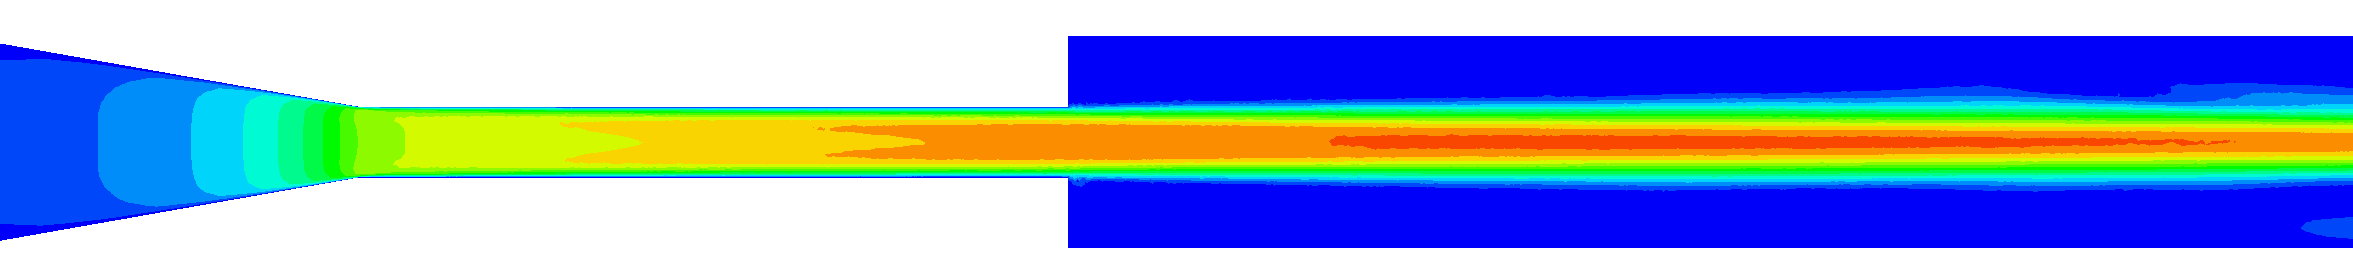
\includegraphics[width=3.2in]{imgs/nozzle_pump/nozzle_fem_fm_cfl1.png}
    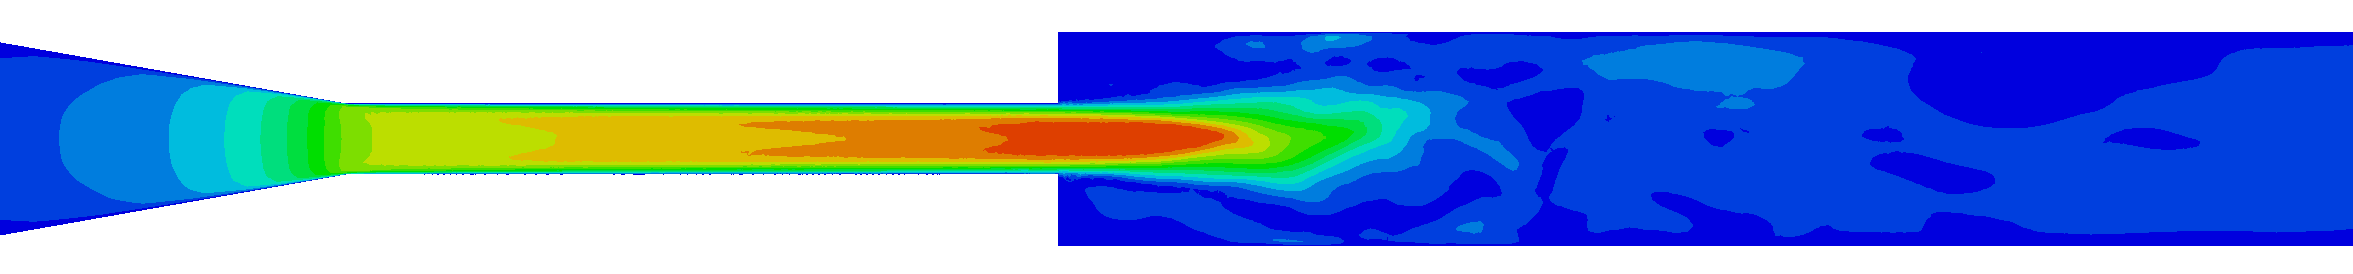
\includegraphics[width=3.2in]{imgs/nozzle_pump/nozzle_fem_fm_cfl5.png}\\
    PFEM-2\\
    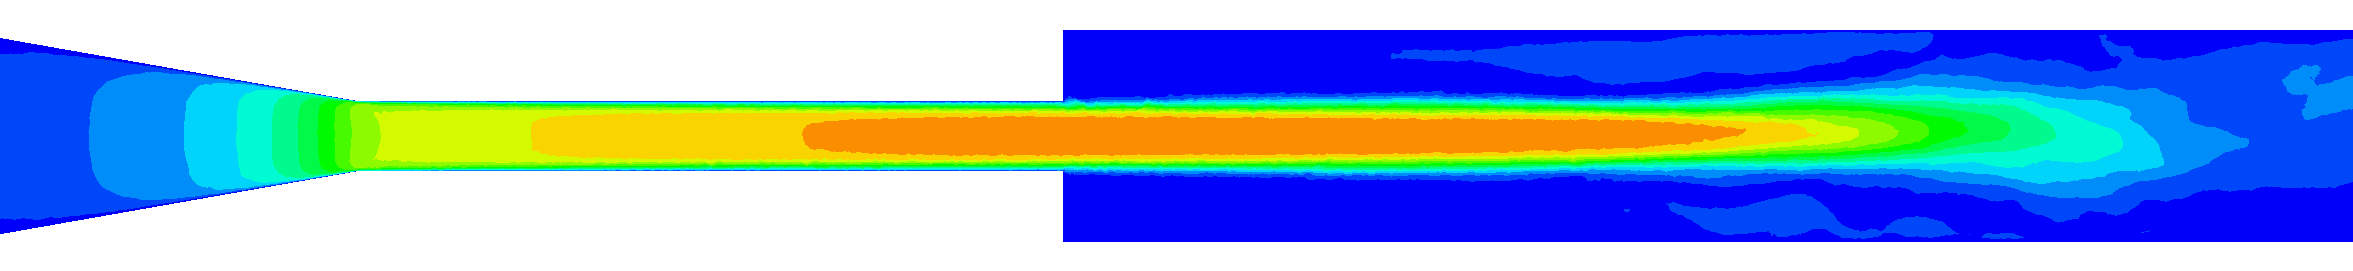
\includegraphics[width=3.2in]{imgs/nozzle_pump/nozzle_pfem_fm_cfl1.png}
    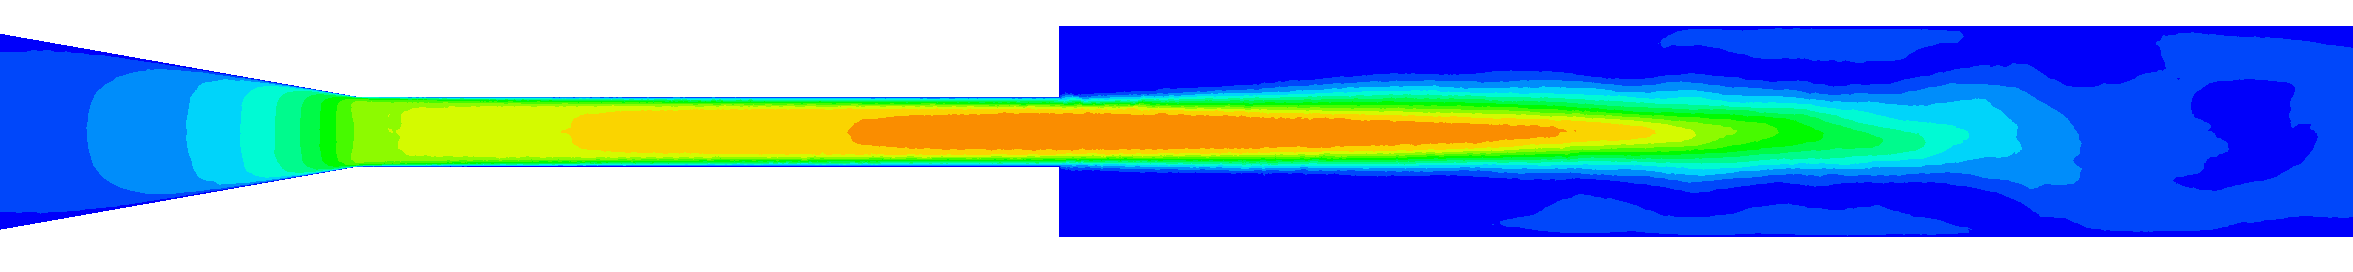
\includegraphics[width=3.2in]{imgs/nozzle_pump/nozzle_pfem_fm_cfl5.png}
    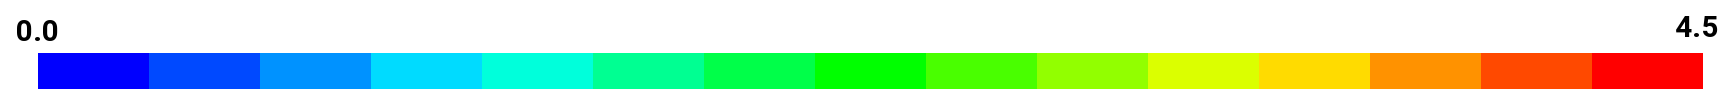
\includegraphics[width=3.2in]{imgs/nozzle_pump/nozzle_legend.png}
    \caption{The obtained time average velocity magnitude distribution in the nozzle at steady state with mesh A using FEM and PFEM-2 with CFL=1 (The 1\textsuperscript{st} and 3\textsuperscript{rd} plots) and CFL=10 (The 2\textsuperscript{nd} and 4\textsuperscript{th} plots). }
    \label{fig:nozzlevelfm}
\end{figure}

\begin{figure}[htbp]
    \centering
    FEM\\
    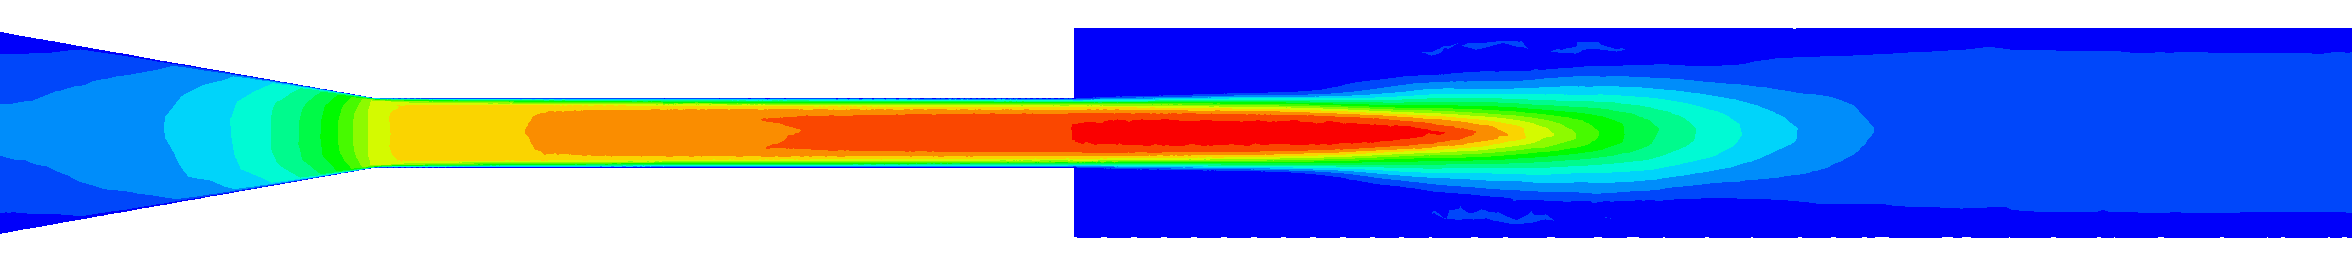
\includegraphics[width=3.2in]{imgs/nozzle_pump/nozzle_fem_pm_cfl1.png}
    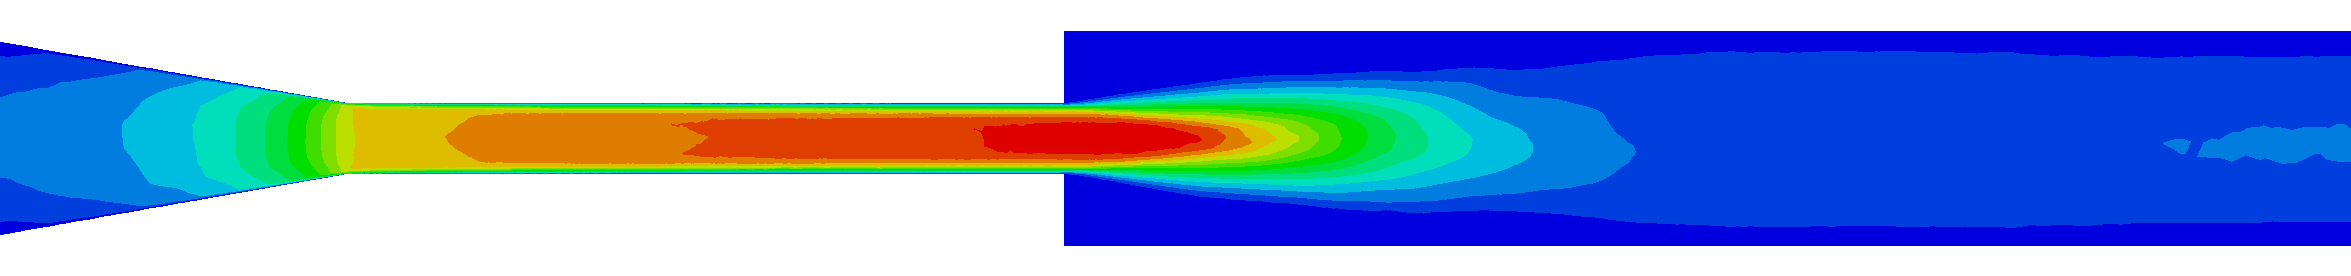
\includegraphics[width=3.2in]{imgs/nozzle_pump/nozzle_fem_pm_cfl10.png}
    PFEM-2\\
    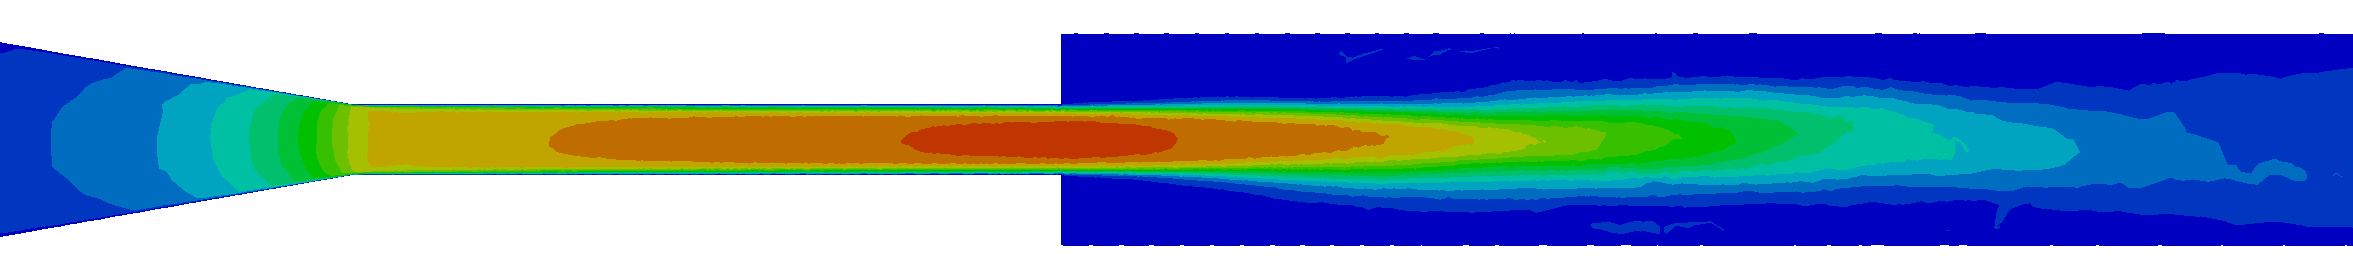
\includegraphics[width=3.2in]{imgs/nozzle_pump/nozzle_pfem_pm_cfl1.png}
    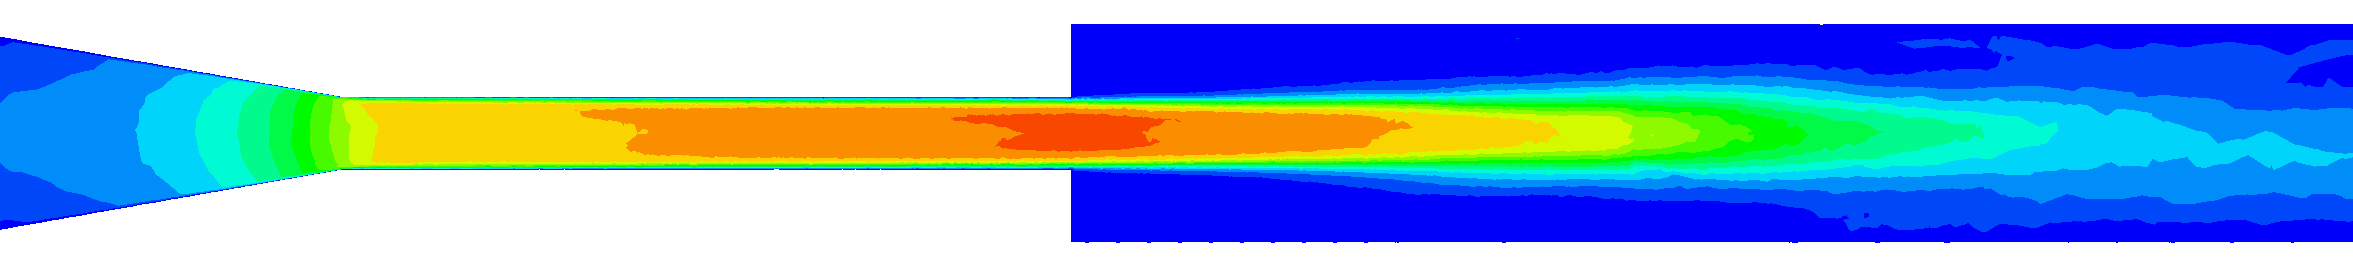
\includegraphics[width=3.2in]{imgs/nozzle_pump/nozzle_pfem_pm_cfl10.png}
    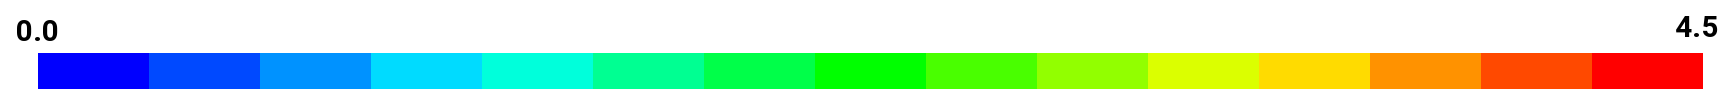
\includegraphics[width=3.2in]{imgs/nozzle_pump/nozzle_legend.png}
    \caption{The obtained time average velocity magnitude distribution in the nozzle at steady state with mesh B using FEM and PFEM-2 with CFL=1 (The 1\textsuperscript{st} and 3\textsuperscript{rd} plots) and CFL=10 (The 2\textsuperscript{nd} and 4\textsuperscript{th} plots).}
    \label{fig:nozzlevelpm}
\end{figure}


\begin{figure}[htbp]
    \centering
    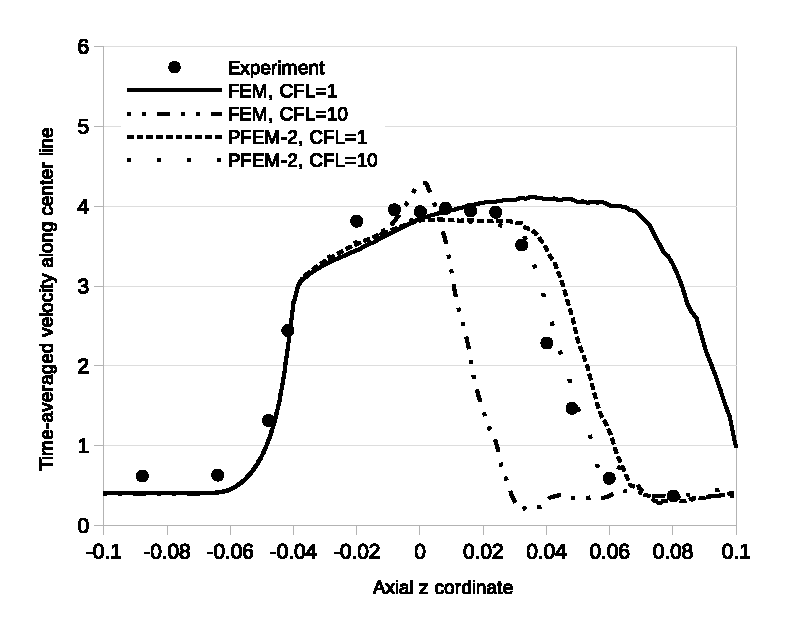
\includegraphics[width=3.2in]{imgs/nozzle_pump/nozzle_midvel_fm2.eps}
    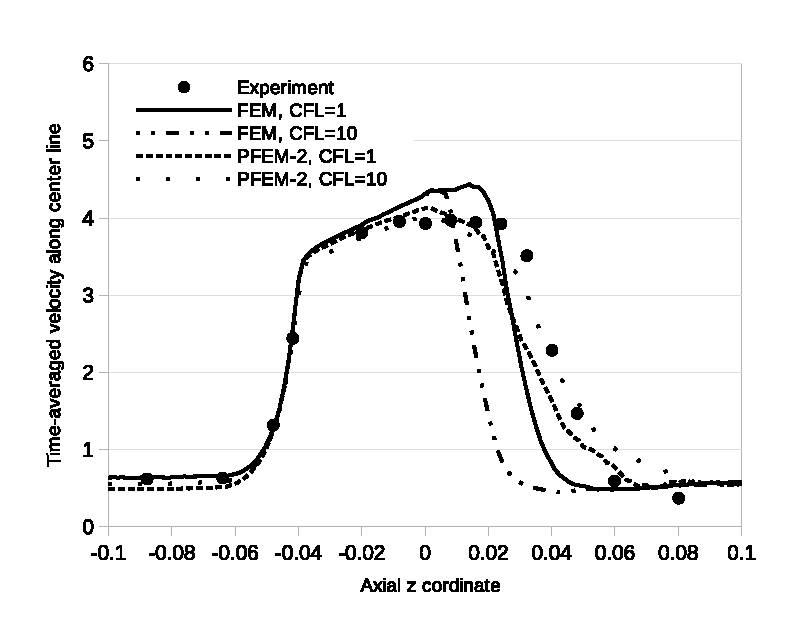
\includegraphics[width=3.2in]{imgs/nozzle_pump/nozzle_midvel_pm2.eps}
    \caption{The distribution of the axial velocity in the nozzle along the center line with mesh A (top) and mesh B (bottom).
%The distribution of the axial velocity in the nozzle along the center line. The top figure depicts the results with mesh A using FEM and CFL=1 (solid), FEM and CFL=5 (dash-dotted), PFEM-2 and CFL=1 (dashed) and PFEM2 and CFL=5 (dotted). The bottom figure depicts the results with mesh B using FEM and CFL=1 (solid), FEM and CFL=10 (dash-dotted), PFEM-2 and CFL=1 (dashed) and PFEM2 and CFL=10 (dotted).
}
    \label{fig:nozzlemidvel}
\end{figure}

\subsection{Blood Pump}

%  pump intro
The geometry of the FDA proposed simplified centrifugal pump is shown in the Fig.~\ref{fig:pumpgeo}. The flow enters the chamber through a curved tube with diameter $12$ mm. The diameter of the inner chamber of the housing is $60$ mm and the thickness is $9$ mm. The rotor inside the chamber has a diameter of $52$ mm and $4$ mm thick, along with four $3$ mm thick straight blades. The chamber is connected with a throat at its outlet, followed by a diffuser to the outlet tube with diameter $12$ mm. The pump flow with flowrate $Q=6$ L/min and rotational speed $3500$ RPM is analyzed. 

\begin{figure}[htbp]
    \centering
    \begin{minipage}[c][2.5in][c]{0.9\linewidth}
        \centering
        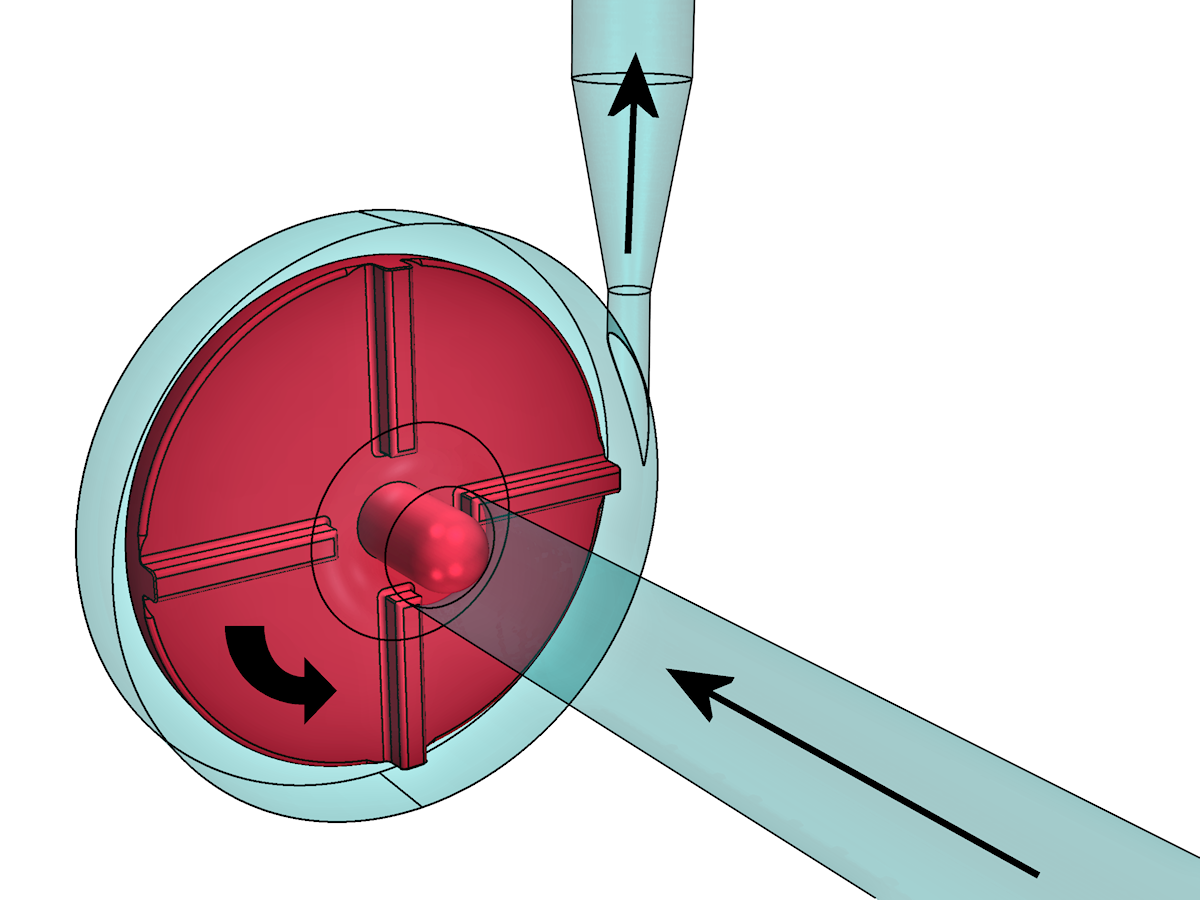
\includegraphics[width=3.2in]{imgs/nozzle_pump/housing_and_rotor.png}
    \end{minipage}
    \begin{minipage}[c][2.5in][c]{0.9\linewidth}
        \centering
        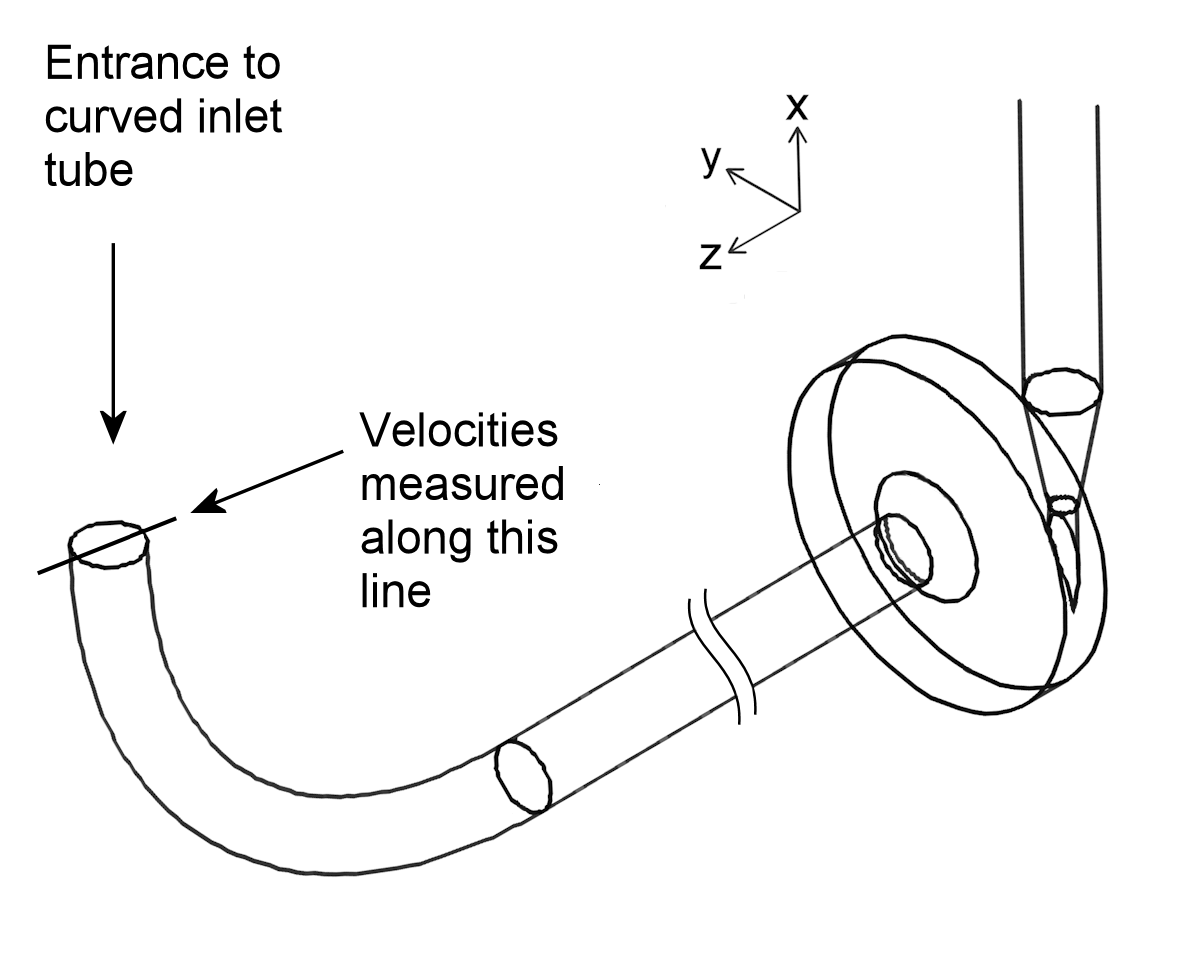
\includegraphics[width=3.2in]{imgs/nozzle_pump/inlet_velcocity_profile_location.png}
    \end{minipage}
    \caption{The pump geometry and the flow direction in the blood pump (top), and the inlet location where the velocity is measured in experiments and where the velocity profile is prescribed in the simulations (bottom).}
    \label{fig:pumpgeo}
\end{figure}

%  pump simulation setup
As to the simulation set up, the velocity distribution is prescribed at the inlet (Fig.~\ref{fig:pumpgeo}), where the velocity profiles are obtained from the experimental measurements using PIV \cite{cpi}. The pressure at the outlet is set to be constant. Since the goal is to predict the flow field after reaching steady state, instead of letting the rotor rotate during simulation, the non-inertial reference frame is applied on the fluid around the rotor. This is because the flow around the rotor at steady state can be analogue to flow experiencing constant angular velocity. Using non-inertial reference frame approximation avoids mesh distortion and frequent remeshing due to rotation. The LES Wall-Adapting Local Eddy-viscosity (WALE) \cite{wale} turbulence model is employed. 

The simulation domain is decomposed into around $1$ million tetrahedral elements. The mesh size is $0.5$ mm on the rotor blades and $0.3$ mm at the outlet of the chamber to the diffuser. The mesh is locally refined around the throat as shown in Fig.~\ref{fig:pumpmesh}. The simulation result is obtained after $8$ rotations when the pump flow already reaches steady state. The time step size is around $10^{-5}$ s in FEM and PFEM-2 simulations at steady state so that the CFL number is less or equal than $1$.  
\begin{figure}[htbp]
    \centering
    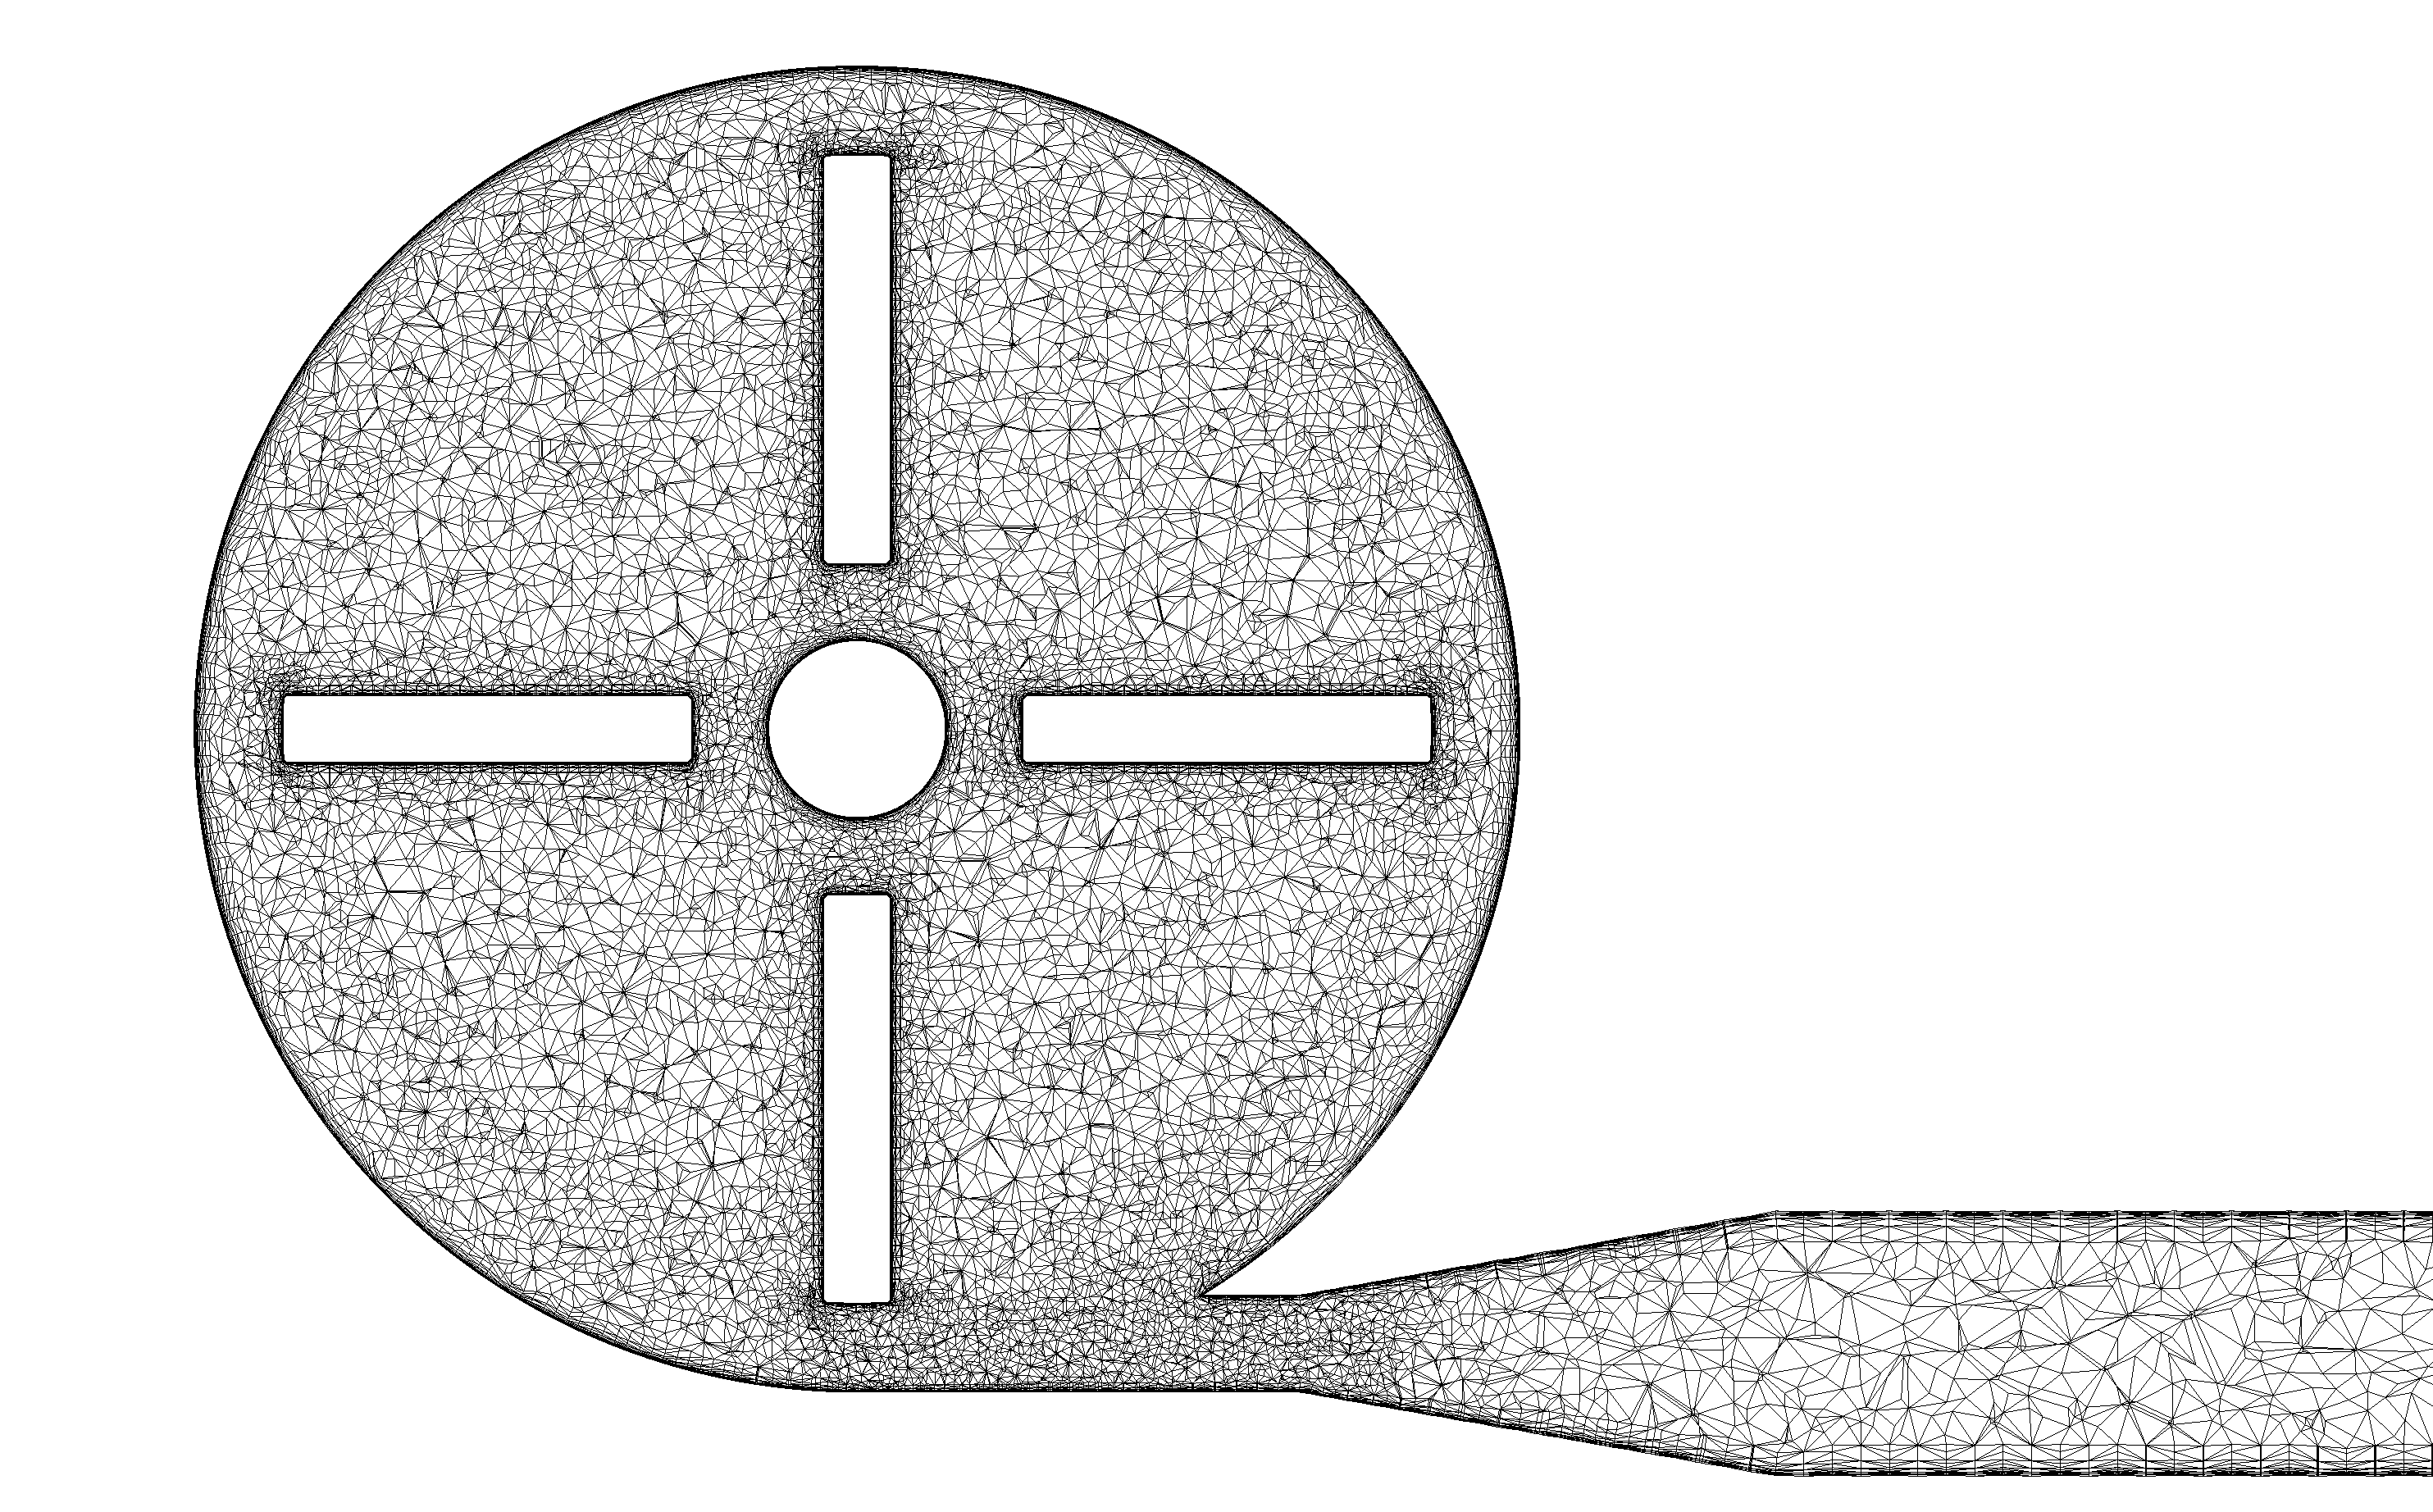
\includegraphics[width=3in]{imgs/nozzle_pump/pump_mesh_2.pdf}
    \caption{The mesh configuration used in the pump flow simulations on the plane coinciding with the mid-axis plane of the outlet diffuser.}
    \label{fig:pumpmesh}
\end{figure}

% pump result & analysis
The pressure difference across the pump obtained by the experiment and the simulations are listed in Table~\ref{tab:pumppres}. Using FEM the discrepancy with experiment is only $3.6$\%. On the other hand, PFEM-2 predicts a lower pressure difference with $14.6$\% discrepancy compared to the experiment. From the distribution of the velocity and pressure fields in the chamber (Fig. \ref{fig:pumpvel} and \ref{fig:pumppres}, the results by PFEM-2 and FEM are qualitatively in accordance with each other. Some discrepancies of the velocity field can be found at the trailing edge near the blade tips, and in the jet flow in the diffuser. 

%it can be observed that the velocity pattern obtained with PFEM-2 is different from FEM. With PFEM-2, the velocity is higher mainly in front of the leading edge of the blade, where with FEM, the velocity is higher at both side of the blade, but more on the trailing edge. \textbf{CHECK:} ***This might be due to in the present PFEM-2 method, the advection and viscous effect are treated separately and sequentially, and an explicit integration scheme is employed. As a result, the particles pushed by the rotor blades have less tendency to turn in chamber than FEM, which can be observed from the streamline plot in Fig.~\ref{fig:pumpsl}. This leads to a larger pressure gradient in the radial direction in order to make particles turn in the chamber. ***

\begin{table}[h]
\caption {Pressure differences across the pump.}\label{tab:pumppres} 
\centering
\begin{tabular}{|c|c|}
\hline
 & Pressure (mmHg) \\ \hline
Experiment \cite{mali_cfd}    & 272.38    \\ \hline
FEM    & 282.40             \\ \hline
PFEM-2    & 232.59          \\ \hline
\end{tabular}
\end{table}

\begin{figure}[htbp]
    \centering
    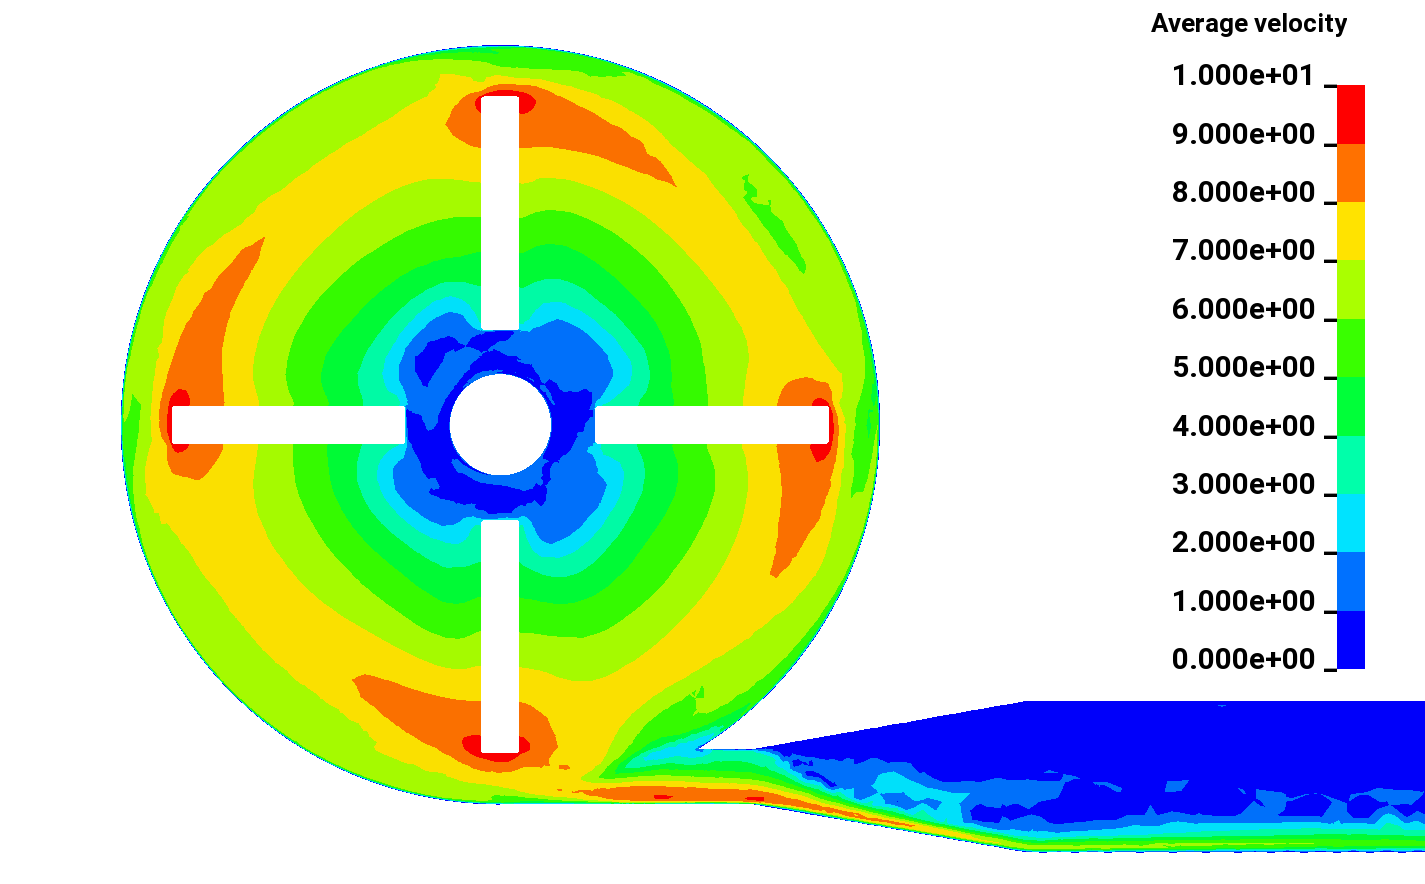
\includegraphics[width=3in]{imgs/nozzle_pump/pumpvel_fem.png}\\
    \vspace{.5cm}
    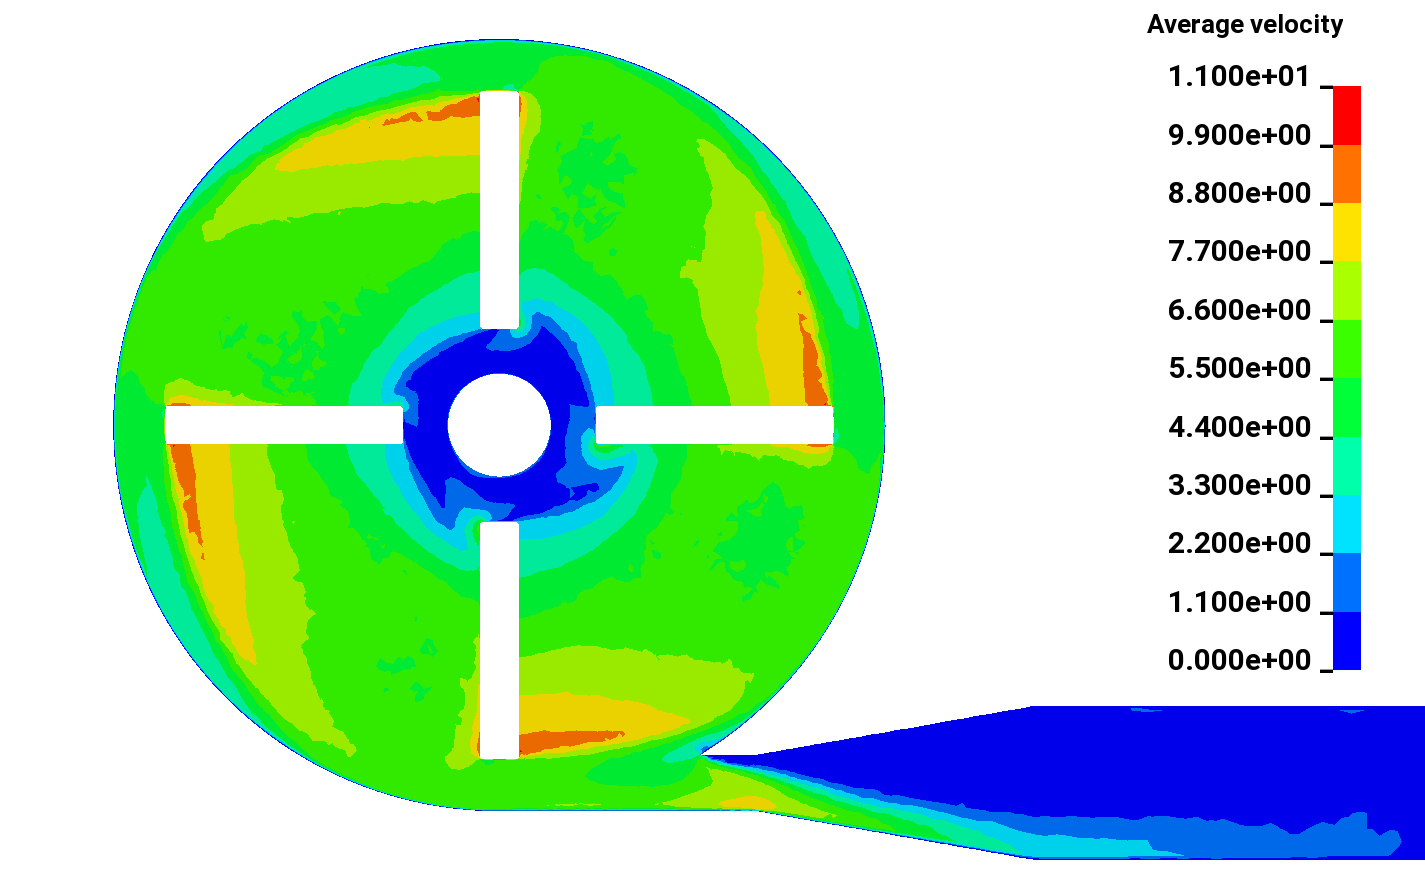
\includegraphics[width=3in]{imgs/nozzle_pump/pumpvel_pfem.png}
    \caption{The velocity magnitude distribution on the plane which coincides to the mid-axis plane of the outlet diffuser using FEM (top) and PFEM-2 (bottom).}
    \label{fig:pumpvel}
\end{figure}

\begin{figure}[htbp]
    \centering
    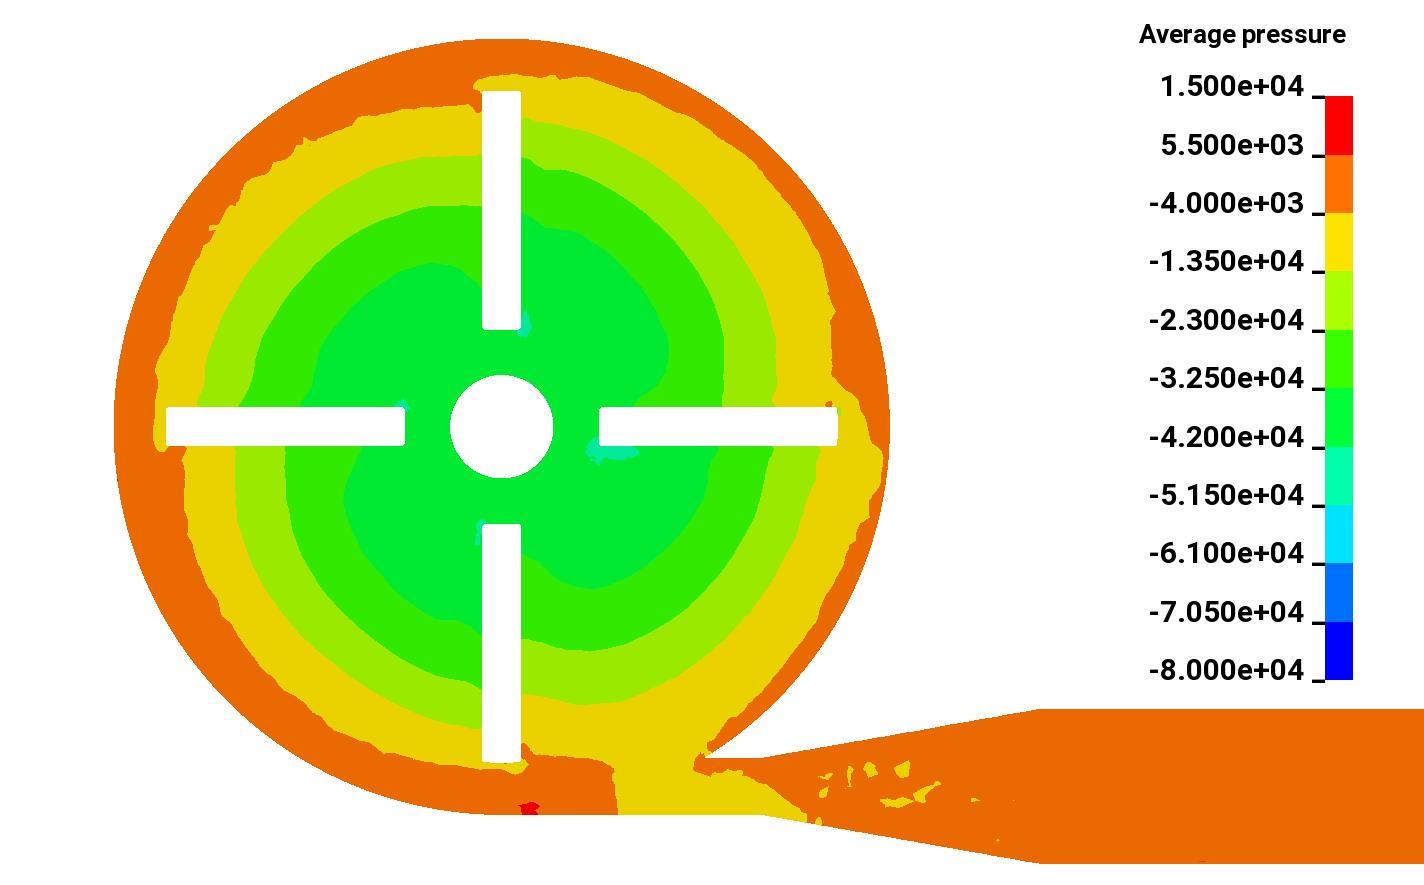
\includegraphics[width=3in]{imgs/nozzle_pump/pumppres_fem.png}\\
    \vspace{.5cm}
    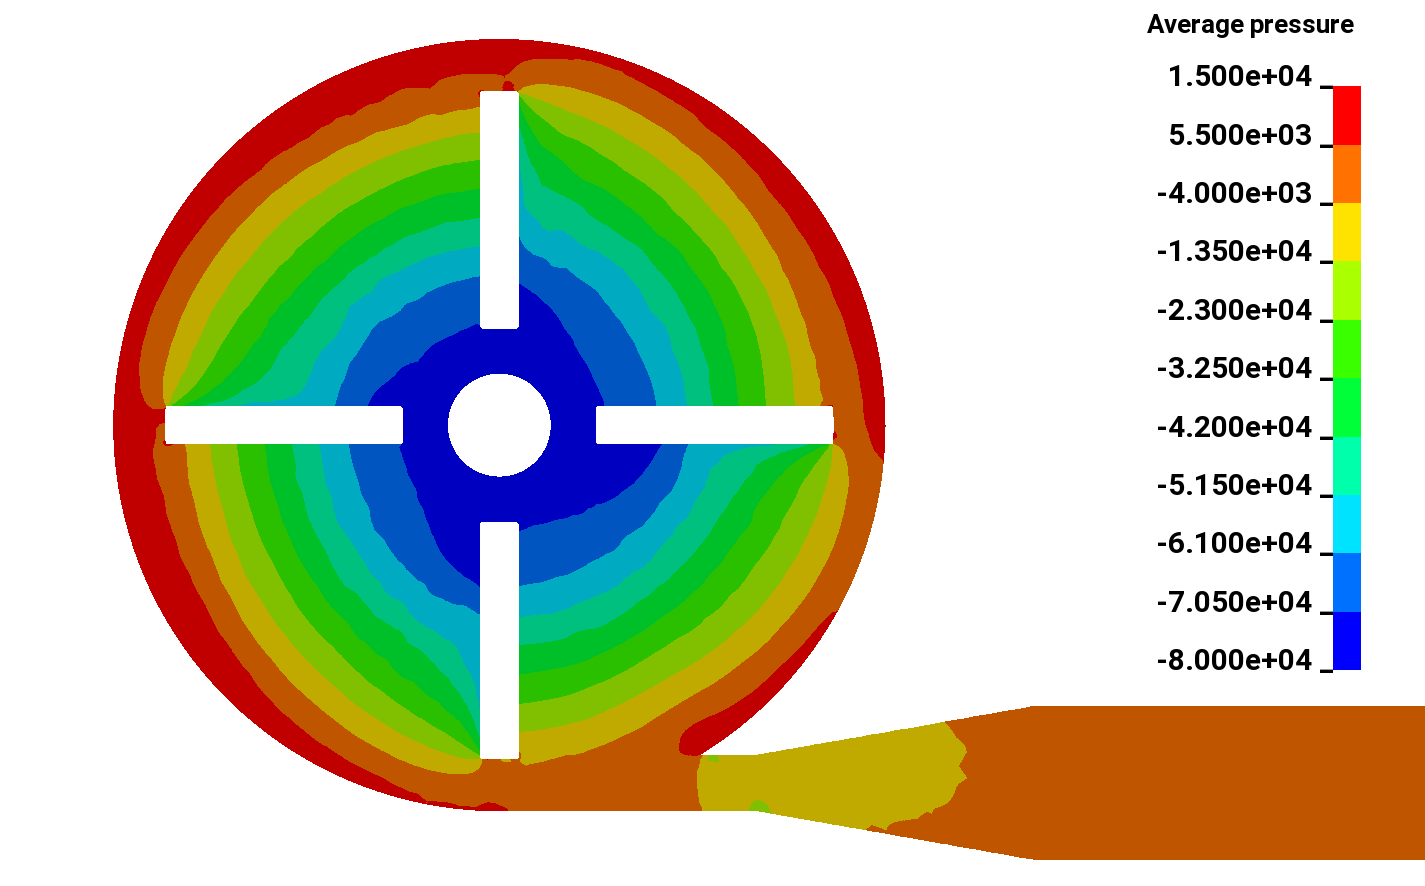
\includegraphics[width=3in]{imgs/nozzle_pump/pumppres_pfem.png}
    \caption{The pressure distribution on the plane which coincides to the mid-axis plane of the outlet diffuser using FEM (top) and PFEM-2 (bottom).}
    \label{fig:pumppres}
\end{figure}

Fig.~\ref{fig:pumpvelprofile} depicts the comparison of the velocity profile in the pump chamber and diffuser compared with the experimental measurements \cite{mali_cfd}. The velocity profile between blades by FEM and PFEM-2 are both in accordance with experiments. In the outlet diffuser, FEM predicts the detached jet leaning more against the outer wall and the velocity magnitude appears to be larger than experiments. The phenomenon may be due to the usage of the non-inertial reference frame approximation since similar velocity distribution in the diffuser can also be observed in most of the other numerical results that use non-inertial reference frame \cite{mali_cfd}.  
 
\begin{figure}[htbp]
    \centering
    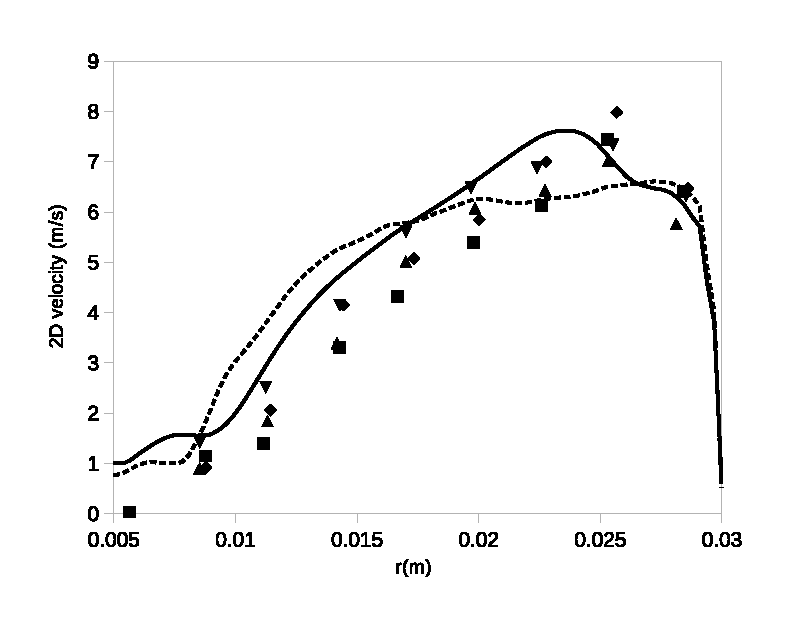
\includegraphics[width=3in]{imgs/nozzle_pump/pump_velblade.eps}\\
    \vspace{.5cm}
    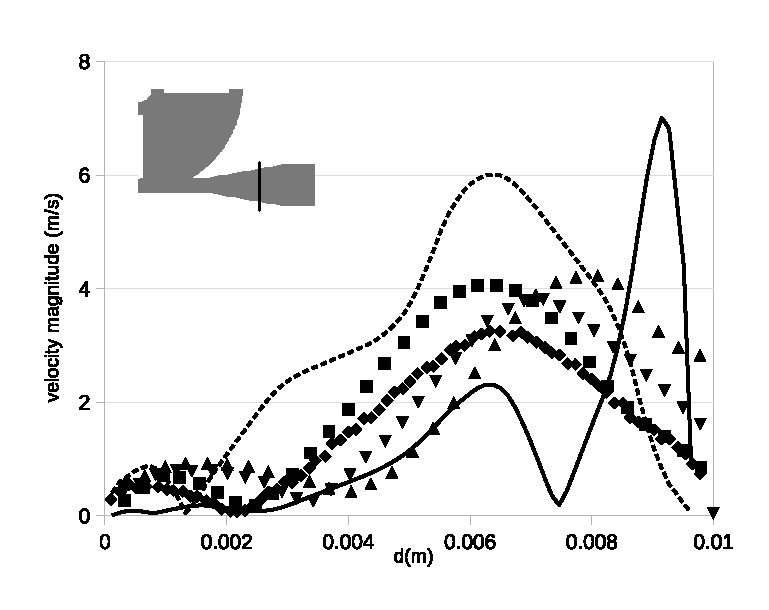
\includegraphics[width=3in]{imgs/nozzle_pump/pump_veldiffuser.eps}
    \caption{The magnitude of the two-dimensional velocity on the same plane as in Figs.~\ref{fig:pumpvel} and \ref{fig:pumppres} with experiments and simulations. Top: velocity profile between two blades where $r$ refers to the distance to rotor center. Right: velocity profile across the outlet diffuser where $d$ refers to distance to the inner wall. $\blacktriangledown$ $\blacktriangle$ $\blacksquare$ $\blacklozenge$: experiments \cite{mali_cfd}. Solid line: FEM. Dashed line: PFEM-2. }
    \label{fig:pumpvelprofile}
\end{figure}
